%%%%%%%%%%%%%%%%%%%%%%%%%%
%%% author : Yamada. T %%%
%%% made for TH series %%%
%%%%%%%%%%%%%%%%%%%%%%%%%%

\documentclass[b5paper,10pt,fleqn] {ltjsarticle}

\usepackage[margin=10truemm]{geometry}

\usepackage{pict2e, graphicx}
\usepackage{tikz}
\usetikzlibrary{intersections,calc,arrows.meta}

\usepackage{amsmath, amssymb, amsthm}
\usepackage{ascmac}
\usepackage{comment}
\usepackage{empheq}
\usepackage[shortlabels,inline]{enumitem}
\usepackage{fancybox}
\usepackage{fancyhdr}
\usepackage{here}
\usepackage{lastpage}
\usepackage{listings, jvlisting}
\usepackage{fixdif}

\usepackage{stmaryrd}
\usepackage[listings]{tcolorbox}
%\usepackage{ascolorbox}
\usepackage{titlesec}
\usepackage{ulem}
\usepackage{url}
\usepackage{verbatim}
\usepackage{wrapfig}
\usepackage{xcolor}
\usepackage{luatexja-ruby}
\usepackage{varwidth}
\usepackage[version=3]{mhchem}
\usepackage{wrapfig}


\usepackage{physics2}
	\usephysicsmodule{ab}
	\usephysicsmodule{ab.braket}
	\usephysicsmodule{ab.legacy}
	%\usephysicsmodule{braket}
	\usephysicsmodule{diagmat}
	\usephysicsmodule{xmat}
	\usephysicsmodule{nabla.legacy}
	\usephysicsmodule{qtext.legacy}

\usepackage[ISO]{diffcoeff}
\difdef { f, s } { D }
{ op-symbol = \mathrm{D} }


\newcommand{\mctext}[1]{\mbox{\textcircled{\scriptsize{#1}}}}
\newcommand{\ctext}[1]{\textcircled{\scriptsize{#1}}}
\newcommand{\ds}{\displaystyle}
\newcommand{\comb}[2]{{}_{#1}\mathrm{C}_{#2}}
\newcommand{\hs}{\hspace}
\newcommand{\vs}{\vspace}
\newcommand{\emphvs}{\vspace{1em}\notag\\}
\newcommand{\ora}{\overrightarrow}
\newcommand{\ol}{\overline}
\newcommand{\oramr}[1]{\overrightarrow{\mathrm{#1}}}
\newcommand{\tri}{\triangle}
\newcommand{\mr}{\mathrm}
\newcommand{\mb}{\mathbb}
\newcommand{\mrvec}[1]{\overrightarrow{\mathrm{#1}}}
\newcommand{\itvec}{\overrightarrow}
\newcommand{\bs}{\boldsymbol}
\newcommand{\ra}{\rightarrow}
\newcommand{\Ra}{\Rightarrow}
\newcommand{\lra}{\longrightarrow}
\newcommand{\Lra}{\Longrightarrow}
\newcommand{\la}{\leftarrow}
\newcommand{\La}{\Leftarrow}
\newcommand{\lla}{\longleftarrow}
\newcommand{\Lla}{\Longleftarrow}
\newcommand{\lr}{\leftrightarrow}
\newcommand{\llr}{\longleftrightarrow}
\newcommand{\Llr}{\Longleftrightarrow}
\renewcommand{\deg}{{}^\circ}
\newcommand{\phbox}{\fbox{\phantom{1\hspace{2em}}}}
\newcommand{\boxnum}[1]{\fbox{\phantom{\hspace{1em}}({#1})\phantom{\hspace{1em}}}}
\newcommand{\boxkana}[1]{\fbox{\phantom{\hspace{1em}}{#1}\phantom{\hspace{1em}}}}
\newcommand{\boxkm}[2]{\fbox{\, {#1}\phantom{\hspace{0.2em}} \,  {#2}}}
\newcommand{\hzw}{\hspace{1\zw}}

\renewcommand{\baselinestretch}{1.25}
\parindent=1\zw

%%入219

\begin{document}
\noindent
\fbox{NewTH4-23} [京都工芸繊維大]

\begin{wrapfigure}{r}{8cm}
  \centering
  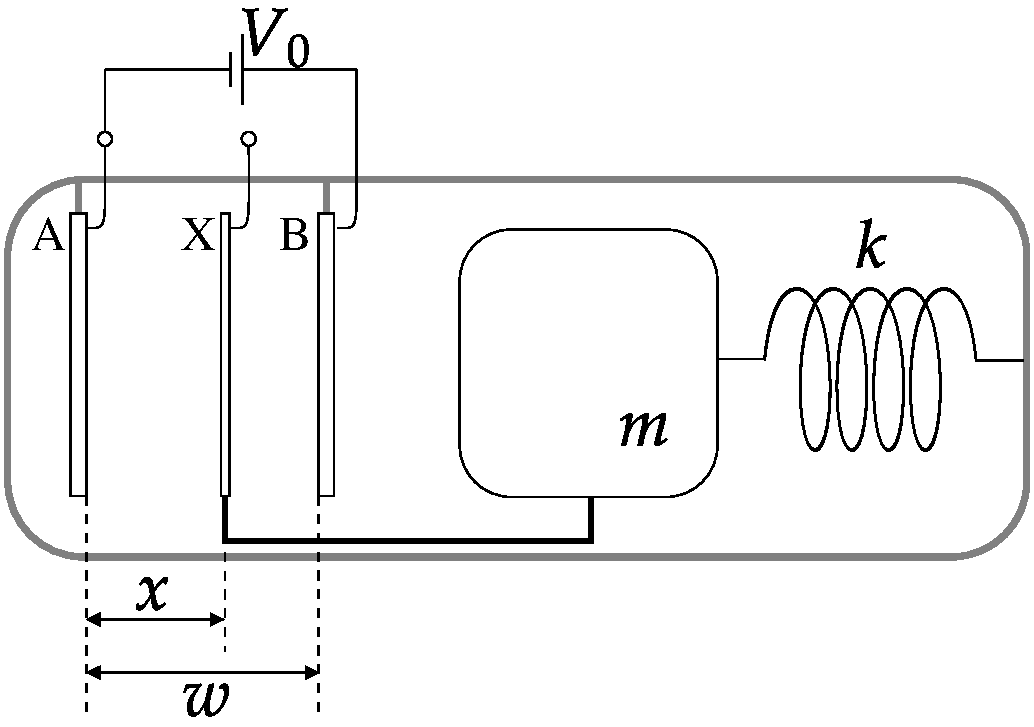
\includegraphics[width=8cm]{fig/fig_4_23.pdf}
\end{wrapfigure}
図は加速度センサー,すなわち加速度を電圧に変換して出力する装置の模式図を示している.ばね定数$k$の軽いばねの一端がケースに固定されており,他端に質量$m$のおもりが取りつけてある.おもりには厚さと質量が無視できる可動極板Xが取りつけてあり,ケースには固定極板AとBが取りつけてある.AとX,およびXとBはそれぞれ平行板コンデンサーⅠ,および平行板コンデンサーⅡを構成している.各極板はいずれも面積が$S$であり,おもりおよびケースから電気的に絶縁されている.ケース内は真空であり,真空の誘電率は$\varepsilon_0$とする.ここで,AとBの間隔を$w$とし,AとXの間隔を$x$とする($x < w$).ばねが自然の長さであるときの$x$の値を$d$とする.センサーを図のように水平に置いたとき,センサーに水平方向の加速度が加わると,センサー内のおもりが慣性力とばねの復元力のつり合う位置に変位する.加速度および力の向きは水平右向きを正とする.

最初,センサーは水平に静止した状態で,ばねは自然の長さであったとする.まず,AとBの間に起電力$V_0$の電池を接続した.以下の(1)〜(3)に答えよ.

\begin{enumerate}[(1)]
  \item AとXの間,およびXとBの間の電界の強さは等しい.その強さを求めよ.
  \item コンデンサーⅠとコンデンサーⅡの合成容量を求めよ.
  \item コンデンサーⅠに蓄えられている電気量を求めよ.
\end{enumerate}

次に,ケースを固定した状態で,おもりを手で動かして変位させた.このときのAとXの間隔を$x$として,以下の(4)〜(6)に答えよ.
\begin{enumerate}[(1), resume]
  \item おもりがばねから受ける力を求めよ.
  \item コンデンサーⅠの電気容量を求めよ.
  \item AとXの間の電位差を求めよ.
\end{enumerate}

この後Xを$x = d$の位置に戻し,静かにおもりから手をはなした.次に,センサーに加速度$a$を与えたところ,おもりが変位してXが移動した.以下の(7),(8)に答えよ.
\begin{enumerate}[(1), resume]
  \item AとXの間隔$x$の値を求めよ.
  \item AとXの間の電位差を求めよ.
\end{enumerate}

この加速度センサーを用いると,(8)の電位差を測定することで加速度$a$を知ることができる.ここで「加速度$a$の変化量に対する(8)の電位差の変化量の比率」を加速度センサーの感度と考え,この感度を大きくするための工夫をしたい.次の問いに答えよ.
\begin{enumerate}[(1), resume]
  \item おもりの質量$m$,ばね定数$k$,電池の起電力$V_0$,AとBの間隔$w$,ばねが自然の長さのときのAとXの間隔$d$のそれぞれの値が感度に与える影響について,
    \begin{enumerate}[label=\mctext{\arabic*}]
      \item 値を大きくすると感度が大きくなる
      \item 値を小さくすると感度が大きくなる
      \item 値を変えても感度は変わらない
    \end{enumerate}

    のいずれであるかを,記号\mctext{1},\mctext{2},\mctext{3}で答えよ.
\end{enumerate}


\end{document}

